\documentclass[twoside,openright,a4paper,12pt]{memoir}
\usepackage[utf8]{inputenc}
\usepackage[T1]{fontenc}
\usepackage{amsfonts}
\usepackage{amsthm}

\usepackage[backend=biber,citestyle=authoryear-comp,hyperref=true]{biblatex}

\pagestyle{ruled}
\setcounter{tocdepth}{3}

\begin{document}
\title{LIGHT MODELLING ON THE GPU}
\author{Michał Siejak}

\frontmatter
\pagenumbering{gobble}
\maketitle
\newpage
\pagenumbering{roman}
\setcounter{page}{2}

\begin{center}
  \LARGE{Oświadczenie}
\end{center}

Ja, niżej podpisany \textbf{Michał Siejak} student Wydziału
Matematyki i Informatyki Uniwersytetu im. Adama Mickiewicza w Poznaniu
oświadczam, że przedkładaną pracę dyplomową pt.:

\centerline{\textbf{Light modelling on the GPU}}

napisałem samodzielnie. Oznacza to, że przy pisaniu pracy, poza niezbędnymi
konsultacjami, nie korzystałem z pomocy innych osób, a w szczególności nie
zlecałem opracowania rozprawy lub jej części innym osobom, ani nie
odpisywałem tej rozprawy lub jej części od innych osób.

Oświadczam również, że egzemplarz pracy dyplomowej w formie wydruku
komputerowego jest zgodny z egzemplarzem pracy dyplomowej w formie
elektronicznej.

Jednocześnie przyjmuję do wiadomości, że gdyby powyższe oświadczenie
okazało się nieprawdziwe, decyzja o wydaniu mi dyplomu zostanie cofnięta.

\newcommand{\kropki}[2]{%
  \vbox{%
    \hbox to #1{\dotfill}%
    \vspace{4pt}%
    \hbox to #1{\hss #2\hss}%
  }
}
\vspace{1cm}
\hbox to \textwidth{%
  \hfil
  \kropki{4cm}{data}%
  \hfil\hfil
  \kropki{4cm}{podpis}%
  \hfil
}
\newpage

\begin{abstract}
\end{abstract}
\newpage

\tableofcontents*

\mainmatter
\chapter{Introduction}
Synthesizing realistic images on computers has been an open research problem in computer science for many years now. Physically-based techniques of light simulation are the most robust methods of achieving appartent photo-realism in rendered images. Up until recently the computational cost of physical light simulation was prohibitive on commodity hardware and as a result the domain of realistic rendering was limited to big computational clusters and specialized graphics workstations.

With the emergence of fully programmable graphics processing units (GPUs) personal computers have been slowly but steadily gaining the needed power to compete with specialized hardware. Modern high-end graphics cards offer computational throughput in orders of teraflops per second and with their highly parallel nature are very well suited for algorithms like raytracing.

In the recent years there has been an ongoing effort to shift professional computational graphics from CPU-based solutions to high end GPUs. Although general purpose programming on GPUs has deemed more challenging to the programmers it often offers exceptional performance surpasing highly optimised CPU-centric algorithms by an order of magnitude.

In this thesis I present the implementation of \emph{Aurora Renderer}: a physically-based Monte Carlo distribution raytracer for modern GPUs. Aurora uses the NVIDIA CUDA technology to accelerate rendering on any GPU with CUDA compute capability 2.0 or higher. Aurora is fully integrated with Autodesk Maya -- an industry standard 3D content creation suite used by professionals in the film, VFX and game development industry.

The full source code, licensed under the MIT open source license, is available on the project page: \url{http://www.siejak.pl/projects/aurora}.
\vfill

\section{Structure of the thesis}
Below is a brief overview of each chapter of the thesis.

\subsection{Chapter \ref{ch:theory} -- Theoretical framework for light simulation}
This chapter introduces the theory behind computational light simulation. Basic mathematical tools are revised and crucial radiometric terms and quantities are defined and related to each other. The bidirectional reflectance distribution function is derived along with several reflection models. The chapter concludes with formulation of the light transport equation describing the energy equilibrium in a 3D scene.

\subsection{Chapter \ref{ch:montecarlo} -- Monte Carlo integration}
Here, a method of numerically solving the light transport equation introduced in the previous chapter is proposed. The basic Monte Carlo integration estimator is derived and the basic instruments for arbitrary distribution sampling are presented to the reader. Several essential 2D sampling strategies are derived and the concept of importance sampling is introduced. The chapter concludes with formulation of the Monte Carlo integration estimator using multiple importance sampling.

\subsection{Chapter \ref{ch:raytracing} -- Distribution ray tracing on the GPU}
This chapter describes the implementation details of Aurora renderer. An overview of high-level architecture is presented followed by introduction of the raytracing algorithm. An effictient ray/scene intersection test is devised using parallel geometry presorting for implicitly representing spatial intersection accelerator. Geometry format optimised for GPU rendering is briefly described and the implementation details of various types of lights and surface shaders are presented. A simple pinhole camera model is introduced. Monte Carlo algorithm for numerically estimating scene illumination and a sampling method for final image reconstruction serve as a conclusion for this chapter.

\subsection{Chapter \ref{ch:results} -- Conclusions and results}
The final chapter of the thesis summarizes rendering results achieved with Aurora. A number of output renders are presented and possible future improvements are discussed.




\chapter{Related work}

\chapter{Theoretical framework for light simulation}

\section{Useful mathematical concepts}

\section{Radiometry and photometry}

\section{Reflection models}

\subsection{The BRDF}

\subsection{Lambertian reflection}

\subsection{Specular reflection}

\subsection{Fresnel reflectance}

\section{The light transport equation (LTE)}


\chapter{CUDA computing model}

\chapter{Implementation details}

\section{Design considerations for the GPU}

\section{Raytracing basics}

\section{Intersection tests}

\subsection{Ray--triangle intersection}

\subsection{Ray--slab intersection}

\section{The No--Memory Hierarchy}

\subsection{Construction}

\subsection{Traversal}

\section{Scene geometry}

\section{Lights}

\subsection{Point light}

\subsection{Directional light}

\subsection{Area light}

\section{Shaders}

\subsection{Shading coordinate system}

\subsection{Lambert shader}

\subsection{Reflective shader}

\section{Rendering}

\subsection{Multiple importance sampling}

\subsection{Estimating direct lighting integral}

\subsection{Handling specular reflections}

\subsection{Antialiasing and filtering}




\chapter{Conclusions and results}
\label{ch:results}

Aurora succesfuly estimates direct illumination in arbitrary scenes via stochastic Monte Carlo raytracing. Achieved performance is promising althorugh not yet adequate for interactive rendering. Autodesk Maya integration makes it a robust and easy to use tool for offline 3D scene visualisation.

\section{Further work}
There is a significant amount of possible future improvements in Aurora.
\begin{itemize}
\item Right now only direct illumination is estimated. Addition of a global illumination algorithm would greatly increase realism by also estimating indirect illumination due to phenomena like diffuse interreflection.
\item Adding support for more complex BRDFs, for example micorfacet models or anisotropic distributions, would be also beneficial to rendering realism.
\item Extending sampling strategies to pseudo Monte Carlo sampling, for example by employing Halton sequences or stratified sampling, would reduce variance and produce images with less noise.
\item Adding multiple GPU support would greatly increase performance on systems with more than one CUDA capable graphics card.
\end{itemize}
\vfill

\section{Example renders}
All images showed in this section were produced with Aurora in Autodesk Maya 2014 on 64--bit Windows 7 system. 

Rendering was performed on a PC equipped with Intel Core i5-3470 processor, 16 GB of RAM and a single NVIDIA GTX 560 Ti graphics card with 1GB of dedicated on--board video memory.

The 3D scene is \emph{Crytek Sponza Atrium}\footnote{\url{http://www.crytek.com/cryengine/cryengine3/downloads}} by Frank Meinl, a widely used test scene for evaluating the performance of rendering algorithms.

Geometry for this scene consists of more than 262,000 triangles. The NMH build time was 1.7 seconds. The images were rendered in full HD 1920x1080 resolution taking 4 image samples per pixel.

\begin{figure}[htb]
  \begin{center}
    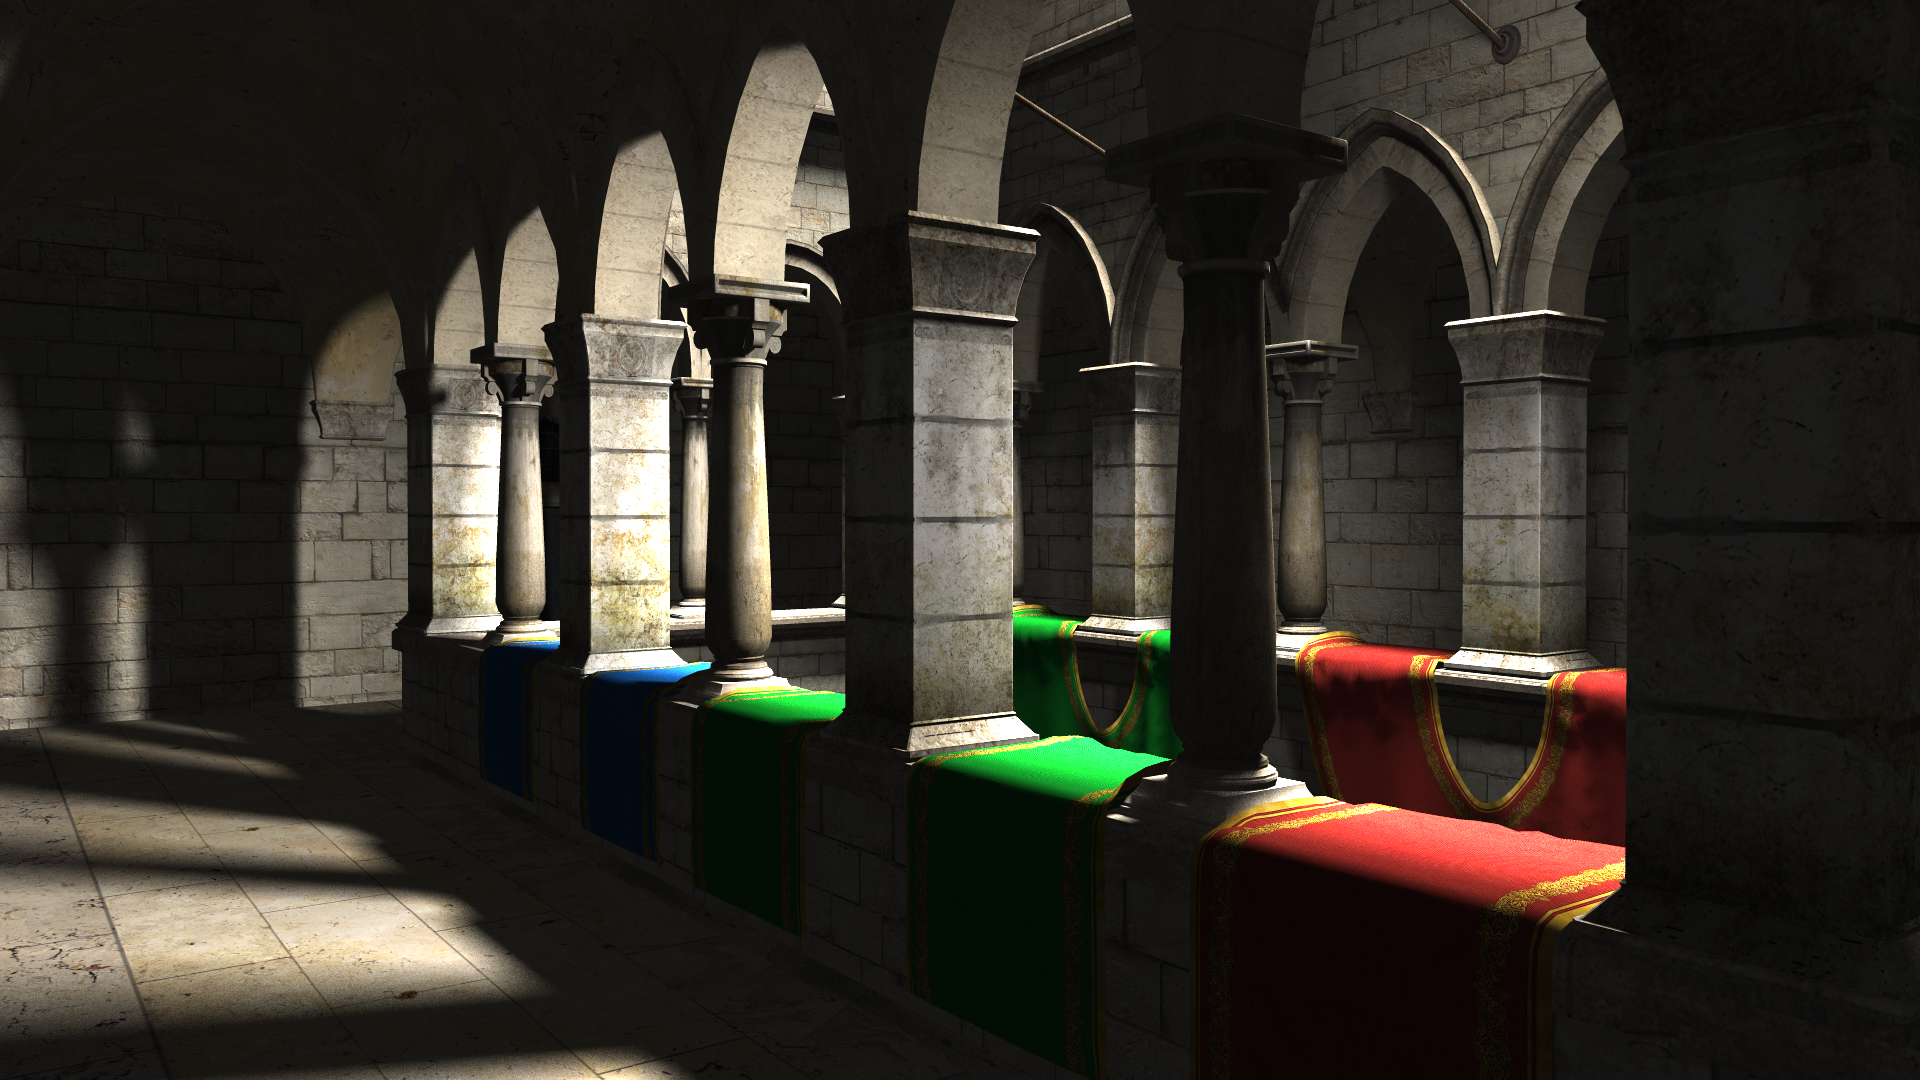
\includegraphics[width=\textwidth]{chapters/results/sponza_softshadows.png}
  \end{center}
  \caption{Test scene illuminated by 3 area lights, with 64 shadow samples per light. Rendering time was about 7 minutes.}
\end{figure}

\begin{figure}[htb]
  \begin{center}
    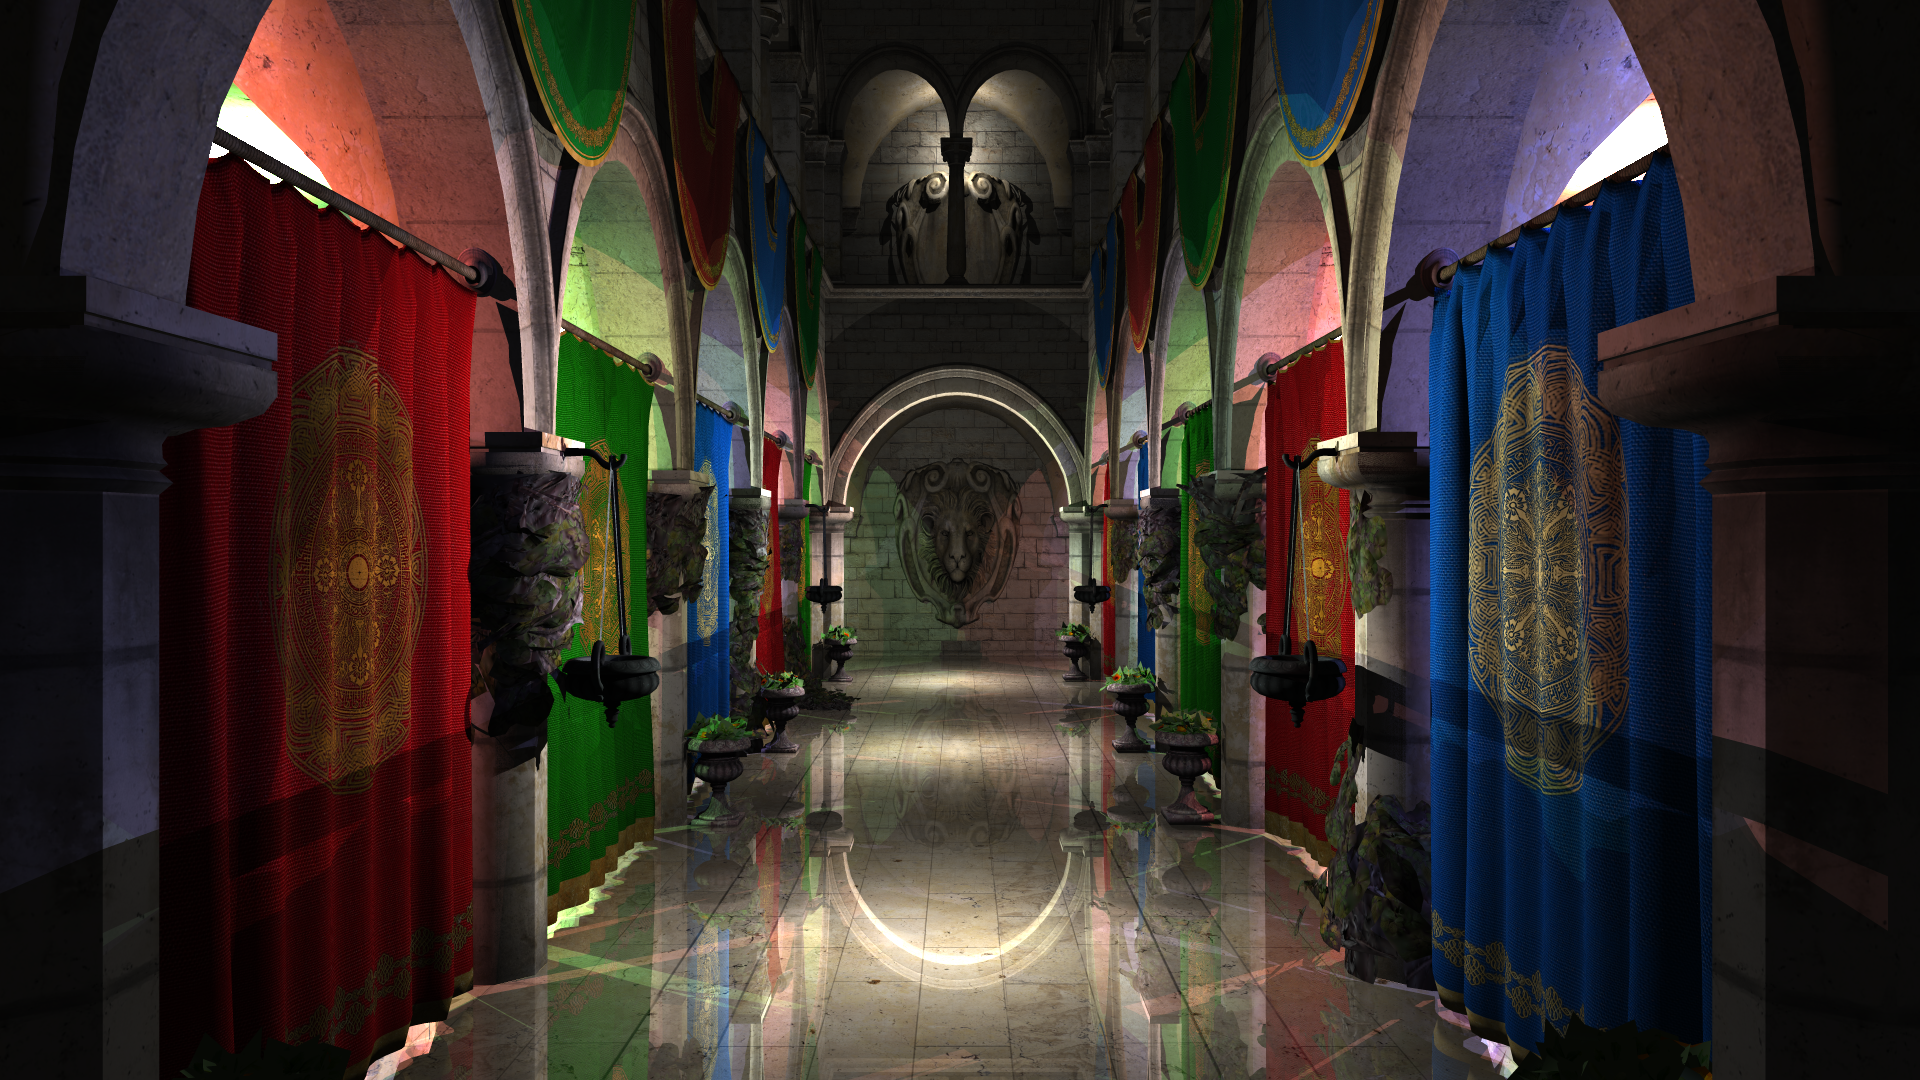
\includegraphics[width=\textwidth]{chapters/results/sponza_manypoint.png}
  \end{center}
  \caption{Test scene illuminated by 14 point lights. Rendering time was about 2.5 minutes.}
\end{figure}

\begin{figure}[htb]
  \begin{center}
    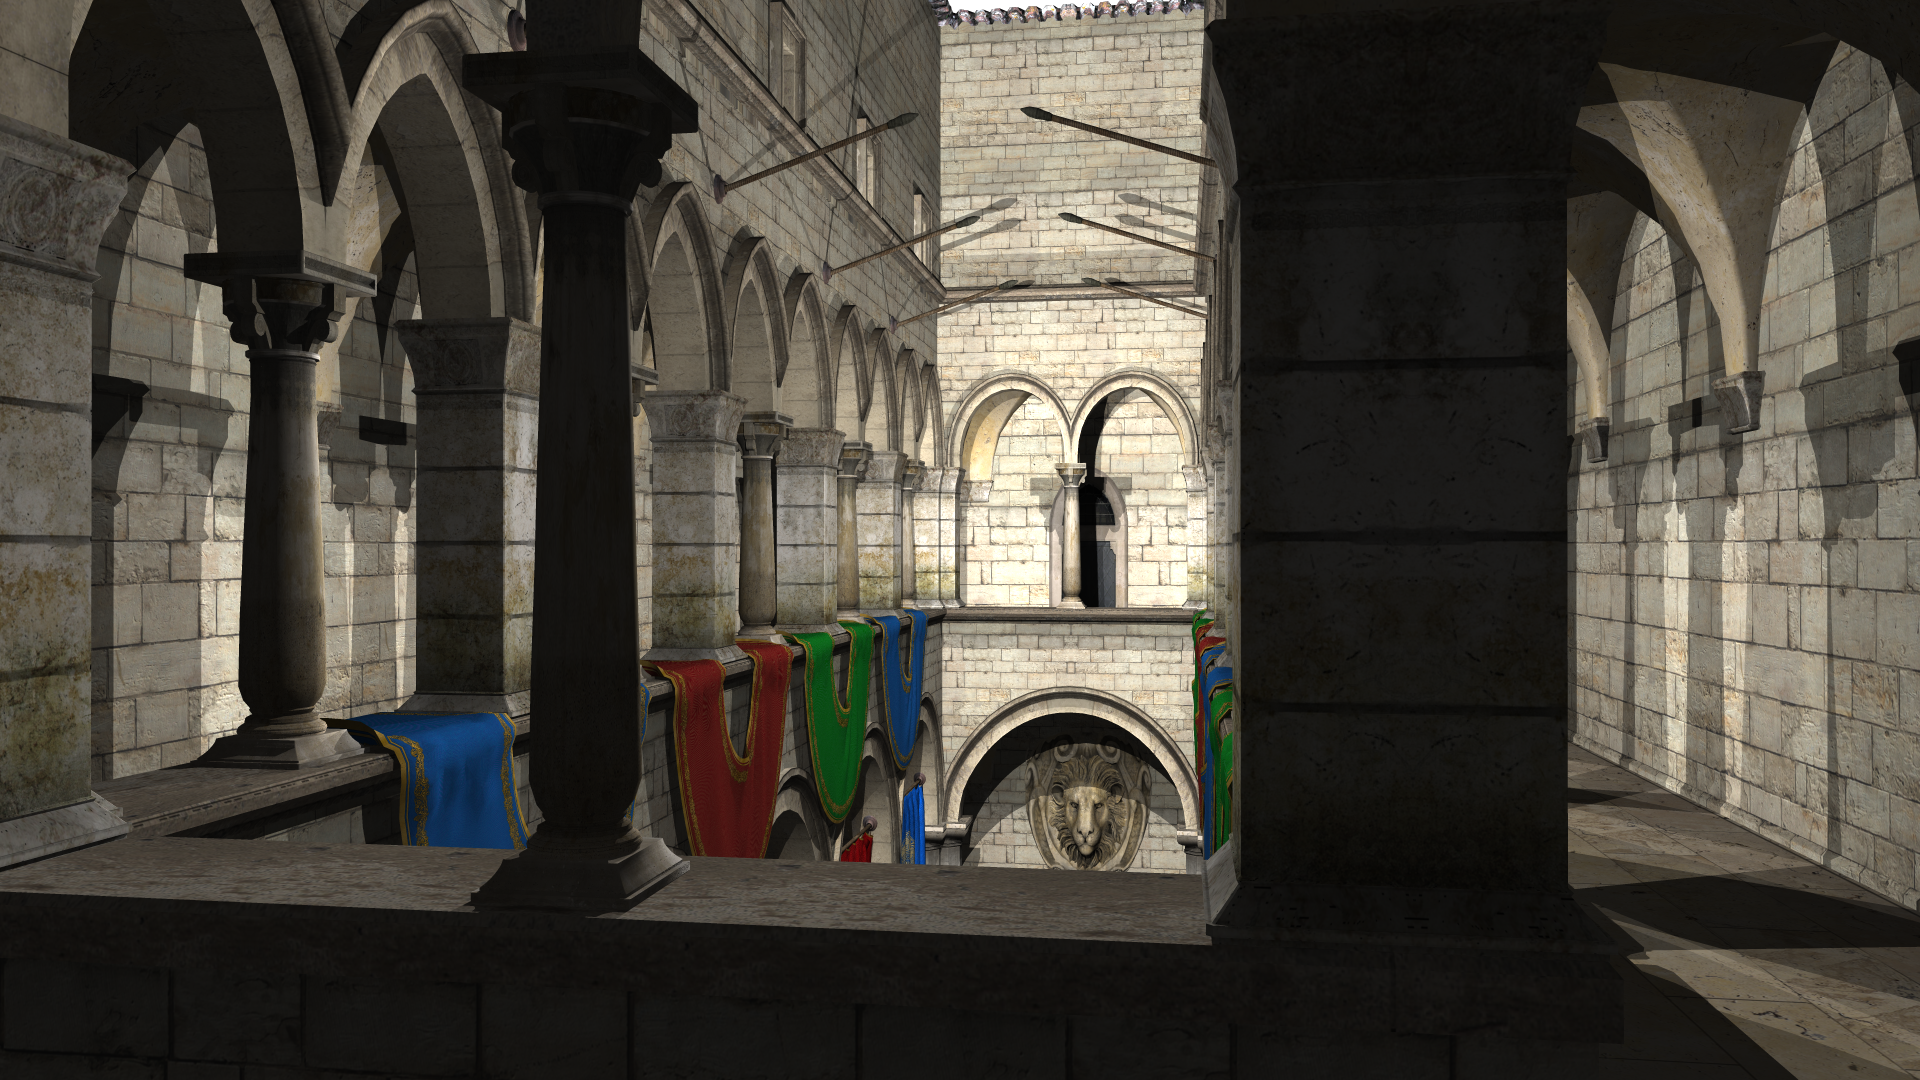
\includegraphics[width=\textwidth]{chapters/results/sponza_point.png}
  \end{center}
  \caption{Test scene illuminated by 3 point lights with no distance falloff. Rendering time was about 18 seconds.}
\end{figure}


\backmatter
\section*{Bibliography}
\printbibliography

\end{document}